% add:  Chernoff had nothing to do with Chernoff Bounds
% add:  Pepsi contest underwritten by Berkshire Hathaway

\documentclass[12pt,twoside]{article}
\usepackage{light}

\begin{document}

%%%%%%%%%%%%%%%%%%%%%%%%%%%%%%%%%%%%%%%%%%%%%%%%%%%%%%%%%%%%%%%%%%%%%%%%%%%%%%%

\lecture{Weird Happenings}{December 7, 2004}

\begin{quotation}
\noindent \textbf{Administrative note:} We've decided to provide an
extra incentive on the final exam: if more than 80\% of the class
scores at least 1.25 times the class average (and the average is
nonzero), then \textbf{everyone gets an \textit{A} for the course!}
We hope that this will encourage you all to study together so that you
all succeed together.
\end{quotation}

%\centerline{\rule{3in}{0.5pt}}

Earlier this term there were 46 people in class, yet no two had the
same birthday, which should happen only about 1 time in 17.  Another
term, students won the Monty Hall game 10 times out of 10.  If
everyone used the optimal ``switch'' strategy, this should happen only
about 1 time in 57.  But some students used the suboptimal ``stay''
strategy and they still won!  This year the Boston Red Sox finally won
the world series after managing to lose for 86 consecutive years.  And
in the recent presidential election, exit polls based on random
sampling showed a Kerry landslide, though Bush got far more votes in
the end!  Weird things happen sometimes.

Yet many computer systems and algorithms are designed assuming that
\textit{weird things won't happen}.  Many web sites are built assuming
that many people will visit occasionally.  So if everyone happened to
visit such a site at the same time, by some weird coincidence, the
system would collapse under the load.  The Quicksort algorithm usually
sorts a list of $n$ items by comparing $O(n \log n)$ pairs of items to
one another.  If $n$ is a million, then this is only a few million
operations.  But the algorithm relies on randomization; so if weird
things happen, Quicksort could take a \textit{half-trillion}
operations instead!  Hash tables are a standard data structure for
rapidly storing and retreiving records.  But, with sufficient bad
luck, accesses can slow to a crawl.  (We'll look at this example more
closely later.)  And the assumption that weird things won't happen is
not only built into computer systems.  What would happen to the phone
system if everyone in America tried to call Topeka at the same time?
Or what if everyone in Cambridge decided to go for ice cream at 7 PM
next Friday?  Our whole society is built around bets that weird things
won't happen!

So to avoid catastrophe, we need mathematical tools to figure out just
how unlikely weird things really are.  That's today's topic.

\section{The New Grading Policy}

Let's return to the special grading policy introduced at the
beginning: if more than 80\% of the class scores at least $1.25$ times
the class average and the average is nonzero, then everyone gets an
\textit{A} for the course.

Suppose there are $n$ students and the class average is $m > 0$.
Let's look at the implications of these conditions, starting with the
definition of class average:
%
\begin{align*}
\text{class average}
    & = \frac{\text{sum of all scores}}{\text{number of students}} \\[0.25ex]
    & > \frac{(0.80 n)\cdot(1.25 m)}{n} \\
    & = m
\end{align*}
%
Thus, the class average must be greater than $m$--- which was defined
to \textit{be} the class average.  This is a contradiction!  In the
same way that not everyone can score above the average, there is no
way more than 80\% can score at least 1.25 times the average.  In
other words, the conditions of the new grading policy can never be
satisfied!  (Sorry.)

\subsection{Markov's Inequality}

Let's recast the analysis of the grading policy in probabilistic
terms.  Suppose that we select a student uniformly at random.  Let the
random variable $X$ denote that student's final exam score.  Then the
class average is just $\ex{X}$, and the conclusion reached above is a
special case of an important general theorem:

\begin{theorem}[Markov's Inequality]
Let $X$ be a nonnegative random variable.  If $c > 0$, then:
%
\[
\pr{X \geq c} \leq \frac{\ex{X}}{c}
\]
\end{theorem}

\begin{proof}
If $\pr{X \geq c} = 0$ or $\pr{X < c} = 0$, then the theorem is
trivially true.  Otherwise, the Total Expectation theorem says:
%
\begin{align*}
\ex{X} &
    = \pr{X \geq c} \cdot \underbrace{\ex{X \mid X \geq c}}_{\geq\ c}
    + \pr{X < c} \cdot \underbrace{\ex{X \mid X < c}}_{\geq\ 0} \\
  & \geq \pr{X \geq c} \cdot c
\end{align*}
%
Dividing the first and last expressions by $c$ proves the theorem.
\end{proof}

For example, if we set $c = (5/4) \ex{X}$ and $\ex{X} > 0$, then the
Markov Inequality says:
%
\[
\pr{X \geq (5/4) \ex{X}} \leq
\frac{\ex{X}}{(5/4)\ex{X}} = \frac{4}{5}
\]
%
In words, the probability that a random student scores $1.25$ times
the class average or better can be at most $80\%$, provided the class
average is greater than zero.

The Markov Inequality puts a limit on weird happenings; in particular,
a nonnegative random variable can deviate far, above its expection
only very rarely.

\subsection{Limitations of the Markov Inequality}

Let's apply the Markov Inequality to a couple more problems:

\begin{itemize}

\item Marilyn vos Savant's IQ is reportedly 228.  How probable is such
an IQ, given that the average is 100?  Let $Q$ be the IQ of a person
selected uniformly at random.  The Markov Inequality says:
%
\[
\pr{Q \geq 228} \leq \frac{\ex{Q}}{228} = \frac{100}{228}
\]
%
So less than half the population is as smart as Marilyn.

\item Let $D$ be the number rolled on a fair die.  How often is a
number greater than or equal to 4 rolled?  Markov's Inequality says:
%
\[
\pr{D \geq 4} \leq \frac{\ex{D}}{4} = \frac{7/2}{4} = \frac{7}{8}
\]
%
Therefore, there is at most a $7/8$ chance of rolling a 5 or 6.

\end{itemize}

\noindent \textit{What's going on here?!}  These two conclusions are
correct, but ridiculously weak.  Far less than half the population has
a 288 IQ, and rolling a 4 or more on a fair die has probabilty
$1/2$--- which is much less than $7/8$!

The difficulty is that the Markov Inequality is fed very little
information, just a random variable's expectation and the fact that
it's nonnegative.  Based on this scanty information, the Markov
Inequality gives the best possible bounds.  Sometimes we don't know
much about a random variable and the Markov Inequality is the only
tool available.  Other times, we can supercharge the Markov Inequality
by incorporating additional data.  We'll return to that approach in a
little while.

%%%%%%%%%%%%%%%%%%%%%%%%%%%%%%%%%%%%%%%%%%%%%%%%%%%%%%%%%%%%%%%%%%%%%%%%%%%%%%%

\section{The Tip of the Tail}

A spaceship has $n$ critical parts.  Let $E_k$ be the event that the
$k$-th part fails on the next flight.  If any critical part fails,
then the spaceship is lost.  This happens with probability:
%
\[
\pr{E_1 \cup \ldots \cup E_n}
\]
%
What can be said about this quantity?

This sort of analysis comes up in the design of any critical system,
where \textit{weird} things can be very \textit{bad} things.  We
define a set of events representing things that can go
catastrophically wrong, and then try to compute the probability that
something does.

%%%%%%%%%%%%%%%%%%%%%%%%%%%%%%%%%%%%%%%%%%%%%%%%%%%%%%%%%%%%%%%%%%%%%%%%%%%%%%%

\subsection{Upper Bound:  The Union Bound}

We can \textit{upper bound} the probability that some critical part
fails using the Union Bound, which follows from the Markov Inequality:

\begin{theorem}[Union Bound]
\label{th:union-bound}
For events $E_1, \ldots, E_n$:
%
\[
\pr{E_1 \cup \ldots \cup E_n} \leq \pr{E_1} + \ldots + \pr{E_n}
\]
\end{theorem}

\begin{proof}
Let $X$ be the number of the events $E_1, \ldots, E_n$ that occur.
Then:
%
\begin{align*}
\pr{E_1 \cup \ldots \cup E_n}
    & = \pr{X \geq 1} \\
    & \leq \frac{\ex{X}}{1} \\
    & = \pr{E_1} + \ldots + \pr{E_n}
\end{align*}
\end{proof}

For example, suppose that the spaceship has 100,000 critical
components and each has a 1-in-a-million probability of failure.  Then
the Union Bound says that the probability that \textit{some} part
fails is at most sum of the failure probabilities of the individual
parts:
%
\begin{align*}
\pr{E_1 \cup \ldots \cup E_{100,000}}
    & \leq \pr{E_1} + \ldots + \pr{E_{100,000}} \\
    & = 100,000 \cdot \frac{1}{1,000,000} \\
    & = \frac{1}{10}
\end{align*}
%
So the flight has at least a 90\% chance of success.

Notice that the Union Bound makes no assumptions about whether the
events $E_i$ are independent or not.  Thus, the Union Bound is great
for conservative risk assessments; if we regard $E_1, \ldots, E_n$ as
``bad events'', then it gives an absolute upper bound on the
probability that some ``bad event'' happens.

%%%%%%%%%%%%%%%%%%%%%%%%%%%%%%%%%%%%%%%%%%%%%%%%%%%%%%%%%%%%%%%%%%%%%%%%%%%%%%%

\subsection{Lower Bound:  ``Murphy's Law''}

Suppose that our spacecraft is a bit more cutting-edge.  Now the
critical components have the following characteristics:
%
\begin{itemize}
\item 10 components each which fail with probability $1/5$.
\item 100 components each which fail with probability $1/40$.
\item 1000 components each which fail with probability $1/200$.
\end{itemize}
%
In this design, components are carefully isolated so that they fail
mutually independently.  Suppose we just put our spaceship on the
launch pad, ``light the candle'', and hope for the best.  What is the
probability that some component fails?  We could crank out the exact
answer, but there's a handy approximation available.

\begin{theorem}[``Murphy's Law'']
\label{th:murphy}
If events $E_1, \ldots E_n$ are mutually independent and $X$ is the
number of these events that occur, then:
%
\[
\pr{E_1 \cup \ldots \cup E_n} \geq 1 - e^{-\ex{X}}
\]
\end{theorem}

\begin{proof}
\begin{align*}
\pr{E_1 \cup \ldots \cup E_n}
    & = 1 - \pr{\overline{E_1 \cup \ldots \cup E_n}} \\
    & = 1 - \pr{\overline{E_1} \cap \ldots \cap \overline{E_n}} \\
%
\intertext{Now we use then fact that $E_1, \ldots, E_n$ are mutually
independent.}
%
    & = 1 - \pr{\overline{E_1}} \cdots \pr{\overline{E_n}} \\
    & = 1 - (1 - \pr{E_1}) \cdots (1 - \pr{E_n}) \\
%
\intertext{Next, we pull out the trusty inequality $1 - x \leq
e^{-x}$, which holds for all $x$.}
%
    & \geq 1 - e^{-\pr{E_1}} \cdots e^{-\pr{E_n}} \\
    & = 1 - e^{-(\pr{E_1} + \ldots + \pr{E_n})} \\
    & = 1 - e^{-\ex{X}}
\end{align*}
\end{proof}

Theorem~\ref{th:murphy} can be regarded as a probabilistic version of
Murphy's Law: \textit{if you expect several things to go wrong, then
something almost certainly will.}  For the spaceship problem, the
expected number component failures is:
%
\begin{align*}
\ex{X}
    & = \pr{E_1} + \ldots + \pr{E_n} \\
    & = 10 \cdot \frac{1}{5} + 100 \cdot \frac{1}{40}
        + 1000 \cdot \frac{1}{200} \\
    & = 9.5
\end{align*}
%
So the probability of a successful flight is at most $e^{-9.5} \approx
0.000075$.  Not a good gamble!

\subsection{The Big Picture}

Let's set the spaceship problem in a broader context.  We have a
sequence of events $E_1, \ldots, E_n$ and $X$ is the number of these
events that happen.  For the second design spaceship design, the
probability density function of $X$ looks something like this:
%
\begin{center}
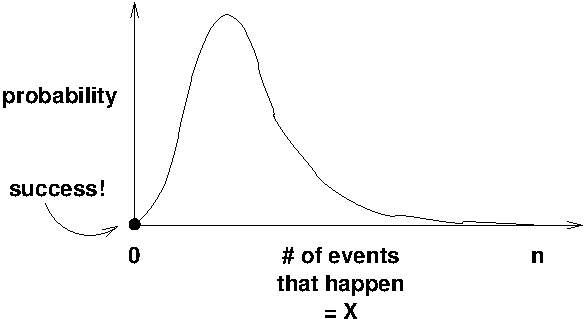
\includegraphics{pdf-x}
\end{center}
%
The spaceship flies successfully only if no critical parts fail; that
is, if $X = 0$.  In terms of the picture, the flight is successful
only at the absolute leftmost point of the distribution.  So in
analyzing the probability that the flight fails, we worked out general
bounds on the probability that we're \textit{not} at the tip of the
tail of the distribution:
%
\[
\underbrace{1 - e^{-\ex{X}}}_{
  \substack{\text{``Murphy's Law''} \\[0.5ex]
            \text{(if $E_1, \ldots E_n$ are independent)}}}
\leq \pr{E_1 \cup \ldots \cup E_n} \leq
\underbrace{\pr{E_1} + \ldots + \pr{E_n}}_{
  \substack{\text{Union Bound} \\[0.5ex]
            \text{(always holds)}}}
\]
%
In particular, Murphy's Law says that if many independent events are
expected to happen, then there's an extremely remote chance that none
of them will.  Thus, being out at the very tip of the tail is
\textit{extremely} weird.  In fact, we're next going to show than
being \textit{anywhere} in either tail of the distribution is pretty
unlikely.

%%%%%%%%%%%%%%%%%%%%%%%%%%%%%%%%%%%%%%%%%%%%%%%%%%%%%%%%%%%%%%%%%%%%%%%%%%%%%%%

\section{Chernoff Bounds}

MIT is admitting a new crop of students.  The Institvte has offered
admission to a few thousand applicants and carefully estimated the
probability that each will accept, based on his or her interests,
enthusiasm, and other likely offers.  This calculation indicates that
the expected number of new students is 1000, which is the ideal
number.  However, MIT must be wary of weird happenings.  If the new
class is too small, then expenses must be divided among fewer
students, forcing tuition up.  If the new class is too large, then
living conditions and classes will be crowded.  What is the
probability that MIT must cope with signficantly fewer or more
students?

Similar problems arise again and again in the analysis of computer
systems and algorithms.  The general theme is that there are many
events that \textit{can} occur, and we need to prove that the number
that actually \textit{do} occur is unlikely to be much greater or much
less than the expected number.  In terms of the probability density
function, we're trying to show that the tails are small:
%
\begin{center}
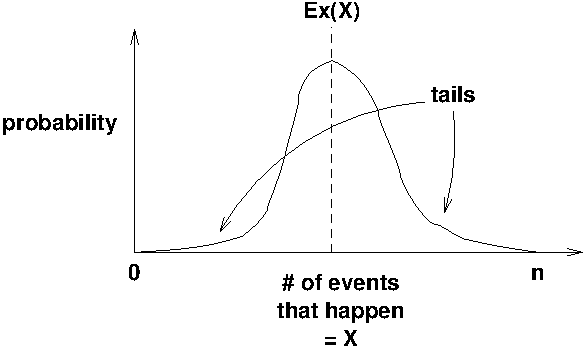
\includegraphics{pdf-x2}
\end{center}
%
If the events are mutually independent, then we can get quick results
to this effect from a powerful set of tools called \term{Chernoff
bounds}.

\begin{theorem}[Chernoff Bounds]
\label{th:chernoff}
Let $E_1, \ldots, E_n$ be a collection of mutually independent events,
and let $X$ be the number of these events that occur.  Then:
%
\begin{align*}
\pr{X \leq (1 - \delta) \ex{X}} & \leq e^{\textstyle -\delta^2 \ex{X} / 2}
    & \text{when $0 \leq \delta \leq 1$} \\[1ex]
\pr{X \geq (1 + \delta) \ex{X}} & \leq e^{\textstyle -\delta^2 \ex{X} / 3}
    & \text{when $0 \leq \delta \leq 1$} \\[1ex]
\pr{X \geq c \ex{X}} & \leq e^{\textstyle -(c \ln c - c + 1) \ex{X}}
    & \text{when $c \geq 1$}
\end{align*}
\end{theorem}

\noindent These are the supercharged Markov Inequalities that we
mentioned earlier.  The proof of this theorem is a bit intricate, so
let's first apply it to the admissions problem.

\subsection{MIT Admissions}

Let $E_k$ be the event that the $k$-th student accepts MIT's admission
offer.  Assume that all such events are mutually independent.  Let $X$
be the number of these events that occur; that is, $X$ is the size of
the incoming freshman class.  The all-knowing admissions office has
determined that $\ex{X} = 1000$.

We can upper bound the probability that the new class contains 900 or
fewer students using the first Chernoff inequality:
%
\begin{align*}
\pr{X \geq 900}
    & = \pr{X < \paren{1 - \frac{1}{10}} \ex{X}} \\
    & \leq e^{- (1/10)^2 \cdot 1000 / 2} \\
    & = e^{-5} \approx 0.0067
\end{align*}
%
On the other hand, we can upper bound the probability that 1200 or
more new students come to MIT using the second inequality:
%
\begin{align*}
\pr{X \geq 1200}
    & = \pr{X > \paren{1 + \frac{1}{5}} \ex{X}} \\
    & \leq e^{- (1/5)^2 \cdot 1000 / 3} \\
    & = e^{-40/3} \approx 0.0000016
\end{align*}
%
If we want to estimate the probability of a complete disaster--- say,
3000 or more students accept--- then we can no longer use the second
inequality; that holds only for deviations up to twice the
expectation.  We must use the third inequality instead.  (Actually,
the third Chernoff inequality always give an answer at least as good
as the second; however, the second is often more convenient.)
%
\begin{align*}
\pr{X \geq 3000}
    & = \pr{X > 3 \cdot \ex{X}} \\
    & \leq e^{-(3 \ln 3 - 3 + 1) \cdot 1000} \\
    & < e^{-1295}
\end{align*}
%
That's pretty unlikely!  

Like the Markov Inequality, a Chernoff bound may not yield the
strongest possible conclusion because it is supplied with very little
information about the random variable $X$.  However, Chernoff bounds
usually give \textit{good} results and they're very easy to apply.  So
Chernoff bounds should among the first tools you reach for when you
need to prove that weird things probably won't happen.

%%%%%%%%%%%%%%%%%%%%%%%%%%%%%%%%%%%%%%%%%%%%%%%%%%%%%%%%%%%%%%%%%%%%%%%%%%%%%%%

\subsection{Proving Chernoff Bounds}

Proving Chernoff bounds takes a good deal of work.  To demonstrate the
techniques involves, we'll prove the third inequality:
%
\[
\pr{X \geq c \ex{X}} \leq e^{\textstyle -(c \ln c - c + 1) \ex{X}}
    \qquad \text{when $c \geq 1$}
\]
%
The argument begins as follows:
%
\begin{align}
\pr{X \geq c \ex{X}}
  & = \pr{c^{X} \geq c^{\textstyle c \ex{X}}} \notag \\
  & \leq \frac{\ex{c^X}}{c^{\textstyle c \ex{X}}} \label{eqn:chernoffbase}
\end{align}
%
In the first step, we exponentiate both sides of the inequality with
base $c$.  The probability remains unchanged because both inequalities
describe the same event.  The second step uses Markov's Inequality.

These two steps illustrate the key idea behind Chernoff bounds.
Remember that Markov's Inequality upper bounds the probability that a
random variable deviates above the mean.  For some probability
distributions, Markov's Inequality gives a tight bound and for others
it doesn't.  Exponentiating before applying Markov's Inequality moves
us to the sweet spot of the Markov Inequality, ensuring that we get
good results.  This isn't the sort of trick you'd immediately think
up, but it works like a charm.

The next task is to find a convenient upper bound on the numerator
in~\eqref{eqn:chernoffbase}.  There are roughly three steps: break the
expression into little pieces, analyze each little piece, and then
assemble them back together again.  Let $I_1, \ldots, I_n$ be
indicators for the events $E_1, \ldots, E_n$.  In these terms, the
number of events that happen is:
%
\[
X = I_1 + \ldots + I_n
\]
%
We'll use this as our starting point:
%
\begin{align*}
\ex{c^X}
    & = \ex{c^{\textstyle \sum_{k=1}^n I_k}} \\
    & = \ex{\prod_{k=1}^n c^{I_k}} \\
    & = \prod_{k=1}^n \ex{c^{I_k}}
%
\intertext{The last step uses the fact that the indicators $I_k$ are
independent and the fact that functions of independent random
variables are themselves independent.  We've now decomposed the
original expression into a product of little pieces, each involving a
single indicator random variable.  The next step is to compute the
expected value of $c^{I_k}$ using the definition of expectation:}
%
    & = \prod_{k=1}^n \pr{E_k} \cdot c^1 +
                       (1 - \pr{E_k}) \cdot c^0 \\
    & = \prod_{k=1}^n 1 + (c-1) \pr{E_k} \\
    & \leq \prod_{k=1}^n e^{\textstyle (c-1) \pr{E_k}} \\
%
\intertext{On the last line we're using the inequality $1 + x \leq
e^x$.  Now we put all the pieces back together again:}
%
    & = e^{\textstyle \sum_{k=1}^n (c-1) \pr{E_k}} \\
    & = e^{\textstyle (c-1) \ex{X}}
\end{align*}
%
Plugging this upper bound into~\eqref{eqn:chernoffbase} gives:
%
\begin{align*}
\pr{X \geq c \ex{X}}
   & \leq \frac{e^{\textstyle (c-1) \ex{X}}}{c^{\textstyle c \ex{X}}} \\
   & = e^{\textstyle -(c \ln c - c + 1) \ex{X}} \\
\end{align*}
%
This is the second Chernoff inequality.  The third inequality follows
by setting $c = 1 + \delta$ and using an approximation based on the
Taylor series of the exponent.  The proof of the first inequality has
a similar structure, but differs in a few details.

A small corollary extends the usefulness of the Chernoff bounds in
further.  Sometimes we don't know $\ex{X}$ exactly, but we at least
know an upper bound.  Fortunately, the second and third Chernoff
inequalities still hold if we use this upper bound instead of the
exact value of $\ex{X}$.

\begin{corollary}
\label{cor:chernoff}
The second and third bounds in Theorem~\ref{th:chernoff} remain valid
when all instances of $\ex{X}$ are replaced by an upper bound on the
expectation of $X$.
\end{corollary}

The proof is a bunch of unenlightening algebra, which we'll omit.

\section{Hashing}

Suppose that we need to store credit histories for a great many
people.  We could create $n = 26^2$ bins labeled $AA, AB, AC, \ldots,
ZZ$.  Then we would store a person's record based on the first two
letters of their name.  For example, the record for ``Lee, Edmond''
would be stored in the bin labeled $LE$.  Then, when we needed to look
up Edmond's credit history, we would only need to search through the
records in bin $LE$, rather than all the records.

In computer science, this trick for rapidly storing and retrieving
records is called \textit{hashing}.  Each record consists of a
\textit{key} and \textit{value}.  A \textit{hash function} maps each
record's key to a bin.  In our example, the keys were names, the
values were credit histories, and the hash function mapped each name
to its first two letters.

The fear in hashing is that one bin somehow ends up with too many
records.  In that case, retrieving any record in the overloaded bin is
time-consuming, since there are so many to search through.  This sort
of imbalance is inevitable if the hash function is chosen poorly.  For
example, the hash function that maps each name to its first two
letters is actually a horribe choice because some two letter prefixes
are quite common ($LE$e, $LE$hman, $LE$ighton) and others extremely
uncommon ($QZ$, $VZ$, $RR$).

An ideal hash function would assign records to bins uniformly and
independently at random.  We can not achieve this goal in a rigorous
sense--- there is really no randomization involved--- but this is
still a decent practical model of a good hash function on typical
data.

So let's assume that $R$ records are hashed to $N$ bins uniformly and
independently at random.  Let's see what our various probability tools
say about the structure of the hash table.

\subsection{The First Collision}

When must there be a bin containing at least two records?

We can answer this question in two ways.  In an absolute sense, the
Pigeonhole Principle says that if there are $R > N$ records, then at
least one of the $N$ bins \textit{must} contains two or more records.

Alternatively, we could regard the records as people and the bins as
possible birthdays.  Then the Birthday Principle says that there is an
even chance that some bin contains two records when:
%
\[
R \approx \sqrt{(2 \ln 2) N}
\]
%
Thus, the first collision is likely to occur when the hash table still
contains very few records.  This can be frustrating.  For example, if
we create a hash table with a million bins, the probability that some
bin contains two records is $1/2$ when the table contains only about
1177 records!

\subsection{\emph{N} Records in \emph{N} Bins}

Suppose that the number of records in our hash table is equal to the
number of bins.  So, for example, we might be storing a million
records in a hash table with a million bins.  What does the table look
like?

Let's first consider a particular bin $B$.  Let $E_k$ be the event
that the $k$-record is hashed to bin $B$.  Since records are hashed
uniformly, $\pr{E_k} = 1/N$.  And these events are independent because
records are hashed to bins independently.

Now let $X$ be the number of these events that happen; that is, $X$ is
the number of records hashed to bin $B$.  The expected value of $X$ is
1 since:
%
\begin{align*}
\ex{X}
    & = \pr{E_1} + \ldots + \pr{E_N} \\
    & = N \cdot 1 / N \\
    & = 1
\end{align*}

We can use Murphy's Law to upper bound the probability that one or
more records are hashed to bin $B$:
%
\begin{align*}
\pr{E_1 \cup \ldots \cup E_N}
    & \geq 1 - e^{\ex{X}} \\
    & = 1 - 1 / e
\end{align*}
%
So $B$ is empty with probability at most $1 / e$.  Thus, the expected
number of empty bins in the whole table is at most $N / e \approx
0.367N$ and this bound is asymptotically tight.

We can upper bound the probability that bin $B$ gets more than $c$
records using the third Chernoff inequality.  Since $\ex{X} = 1$, this
has a simple form:
%
\begin{align*}
\pr{X \geq c} \leq e^{\textstyle -(c \ln c - c + 1)}
\end{align*}
%
How high must we set the threshold $c$ so that $\pr{X > c}$, the
probability that $c$ or more records are stored in bin $B$, is still
small?  Let's try $c = \ln N$:
%
\begin{align*}
\pr{X \geq \ln{N}}
    & \leq e^{\textstyle -(\ln N \ln \ln N - \ln N + 1)} \\
    & = \frac{1}{N^{\displaystyle \ln \ln N - 1 + 1 / \ln N}}
\end{align*}
%
The dominant term in the exponent is $\ln \ln N$, which tends to
infinity for large $N$.  So this probability goes to zero faster than
the inverse of any polynomial in $N$.  So, asymptotically, it is very
unlikely that any bin contains $\ln n$ or more records.

In fact, the probability that bin $B$ contains more than $c$ records
is still less than $1 / N^2$ when $c = e \ln N / \ln \ln N$.  (This
``log over log-log'' function comes up pretty often.  Say ``nice
function'' and let it sniff you.  Then give it a pat, and you'll be
friends for life.)  By the Union Bound, the probability that there
exists \textit{some} bin containing more than $c$ records is at most:
%
\begin{align*}
\pr{\text{some bin has } \geq \frac{e \ln N}{\ln \ln N}}
    &\leq \pr{\text{bin 1 does}} + \ldots + 
          \pr{\text{bin $N$ does}} \\
    & \leq N \cdot \frac{1}{N^2} \\
    & = \frac{1}{N}
\end{align*}
%
So, for example, if we put a million records into a million-bin hash
table, then there is less than a 1-in-a-million chance that any bin
contains $15 > e \ln 10^6 / \ln \ln 10^6$ or more records.

\subsection{All Bins Full}

A final question: what is the expected number of records that we must
add to a hash table in order for every bin to contain at least 1
record?

This is a restatement of the Coupon Collector problem, which we
covered last time.  The solution is $R = N H_n \approx N \ln N$.  For
example, if the hash table contains $N = 1,000,000$ bins, then we must
add about $13.8$ million records to get at least one record in every
bin.

Unless something weird happens.

%%%%%%%%%%%%%%%%%%%%%%%%%%%%%%%%%%%%%%%%%%%%%%%%%%%%%%%%%%%%%%%%%%%%%%%%%%%%%%%

\end{document}
